\documentclass{article}

\usepackage{Mathematics}
\usepackage{longtable}
\usepackage{booktabs}
\usepackage{textcomp}

\newcommand{\tra}{\textrightarrow\ }

% === TEXT ===
\pdftitle{Windpower and Ecotechnology}
\title{\textbf{Windpower and Ecotechnology\\HSLU, Intensive week}}
\author{Matteo Frongillo}
\date{}

\begin{document}

\maketitle
\tableofcontents
\pagebreak

\part{Environmental Impact Assessment}
\section{Environmental benefits vs. environmental impact}
\subsection{Environmental benefit}
Benefits of windpower:
\begin{itemize}
    \item Zero-emissions energy;
    \item Manutention between 10 and 20 years;
    \item Energy produced by wind is normally always available and free;
    \item Relative quick building;
    \item Gains in environmental (natural) services or ecological properties
        by certain actions.
\end{itemize}

\subsection{Environmental impact}
Energy sector in general:
\begin{itemize}
    \item Energy sector as a whole is rated to have negative influence on the environment;
    \item Various processes involved in the energy chain generate environmental stress;
    \item Energy chain: Raw materials procurement \tra Conversion to energy/electricity \tra Energy/electricity use;
    \item Main pollutants causing environmental stress are:
    \begin{itemize}[label=$\circ$]
        \item Airborne emissions (PM and gaseous);
        \item GHGs;
        \item Liquid waste discharges on water and soil;
        \item Solid waste;
    \end{itemize}
    \item Not all energy sources have the same environmental impact or natural resource depletion capability;
    \item How to quantify/rate environmental impacts/benefits on ecosystem?
    \begin{itemize}[label=\textrightarrow]
        \item Environmental benefits are mainly expressed in terms of avoided environmental impacts (e.g.: gains in environmental services or ecological properties attained by using e.g. wind power)
    \end{itemize} 
\end{itemize}

\section{Environmental impact assessment (EIA)}
\begin{itemize}
    \item Identification and qualification of impacts on ecosystems;
    \item Detection and reduction of environmental impacts within entire
        lifetime of energy systems;
    \item EIA should allow to compare different energy sources.
\end{itemize}

\subsection{Field of use}
EIA is used as a planning procedure or decision-making instrument:
\begin{itemize}
    \item Planning procedure:
    \item Decision-making instrument: 
\end{itemize}

EIA can help to achieve:
\begin{itemize}
    \item 1
    \item 2
    \item 3
    \item 4
\end{itemize}

\subsection{Definition}
EIA is the formal process for:
\begin{itemize}
    \item Identifying \underline{likely} impacts (effects) of activities
    (projects) on the environment, human health, and economy;
    \item Identifying measures to mitigate and monitor these impacts.
\end{itemize}

\section{Impact}
\subsection{Definitions}
\subsubsection{Impact}
Impact is the deviation (change) from the baseline situation that
is caused by the activity\\
\tra Impacts can only be quantified knowing the baseline situation.

\subsubsection{Baseline situation}
The baseline situation is the existing environmental condition, in absence of activity.

Baseline situation is not a simple snapshot, thus natural variability
and current trends need to be considered.

\subsubsection{Environmental components}
Various environmental components may be of interest to characterize the baseline situation:
\begin{itemize}
    \item Water (quality, quantity, use, accessibility, ...);
    \item Soil (nutrient concentration, crop productivity, erosion, salinity, ...);
    \item Biodiversity (flora and fauna, populations, habitat, ...);
    \item Environmental health (existing diseases, pathogens, ...);
    \item Special ecosystems (key species, endangered species).
\end{itemize}

\subsection{Types of impacts}
EIA doesn't treat all impacts equally:\\
\tra Focus is set on the most significant impacts which might
change project outline/direction.

Some types of impacts:
\begin{itemize}
    \item Direct vs indirect impacts:
        \begin{itemize}
            \item Direct: What wind power plants do to the nearby environment (e.g.: noise pollution);
            \item Indirect: What wind power plants do to the planet;
        \end{itemize}
    \item Short-term vs long-term impacts;
    \item Adverse vs beneficial impacts;
    \item Cumulative impacts (synergistic effects).
\end{itemize}

\subsection{Impact measure units}
Impacts can be measured in numerous ways:
\begin{itemize}
    \item Intensity (e.g.: ppm, Hertz, Watt, ...);
    \item Probability (occurrence);
    \item Spatial extent (magnitude);
    \item Duration:
    \begin{itemize}
        \item 1
        \item 2
        \item 3
        \item 4
    \end{itemize}
    \item Reversibility.
\end{itemize}

\subsection{Application fields}
...

\section{Benefits of implementing EIA in project}
...

\section{EIA process}
\begin{center}
    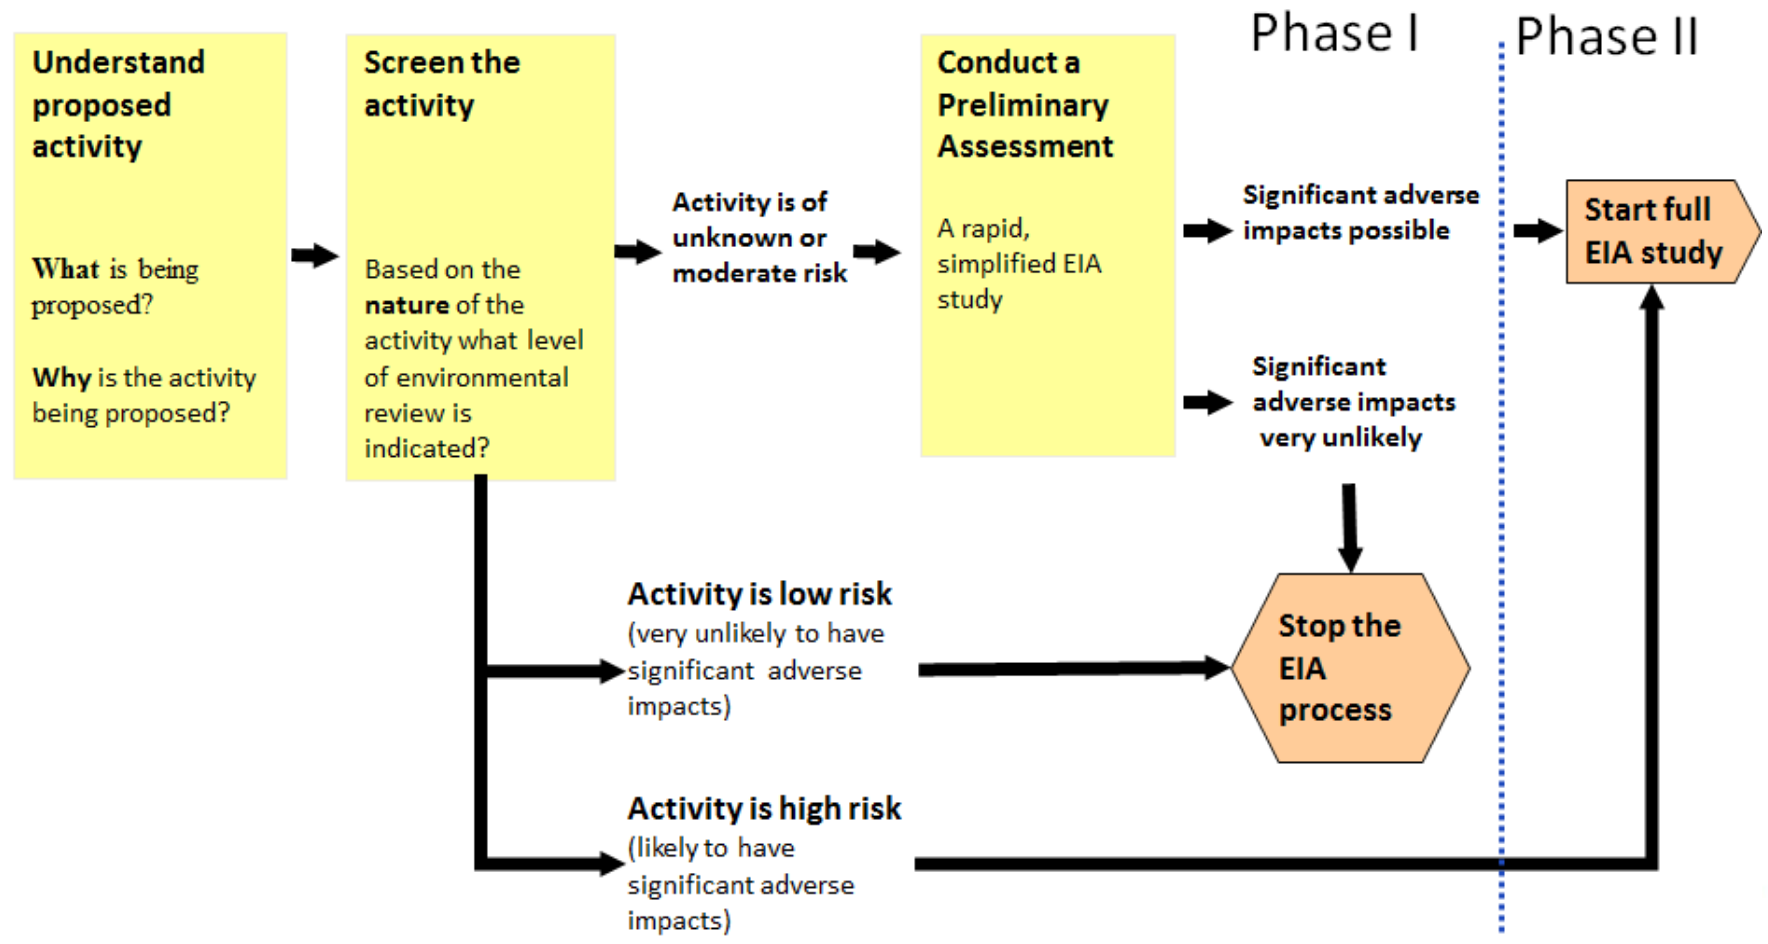
\includegraphics[width=.9\textwidth]{media/EIA_process.png}
\end{center}

\subsection{Phase \rom{1} - Initial inquiries}
\subsubsection{Understand proposed activity}
\begin{enumerate}
    \item EIA processes begin with \underline{understanding why} an activity is proposed:
    \begin{itemize}
        \item Answer requires definition of development objective (D.O.);
        \item Understanding D.O. allows to identify environmentally sound alternatives.
    \end{itemize}

    D.O. example:
    \begin{itemize}
        \item Building a road \tra NOT a D.O.
        \item Increasing access to a certain area \tra D.O.
    \end{itemize}
    
    \item Understanding \underline{what is being proposed} including associated actions:
    \begin{itemize}
        \item Primary activity (e.g.: construction of a road);
        \item Associated actions (e.g.: clearing of forest, soil drainage, ...).
    \end{itemize}
\end{enumerate}

\subsubsection{Screen the activity}


\newpage
\part{Environmental impacts - onshore}
\section{Stakeholders analysis}
\subsection{Definition}
SA is a methodology used to ``facilitate institutional and policy reform processes by accounting
for and often incorporating the needs of those who have a ``stake'' or an interest in the reforms
under consideration'' (World Bank)

SA is ``a tool for assessing different interest groups around a policy issue or intervention, and
their ability to influence the final outcome'' (FAO)

SA is applied to identify and sort stakeholders that are likely to affect or be affected by a
proposed action (e.g. project), according to their impact and the impact the action might have
on them

\subsection{Goals}
\begin{enumerate}
    \item Development of a strategic view of the human and istitutional landscape:
    \begin{itemize}
        \item Including the relationships between different stakeholders;
        \item Issues different stakeholders care about most;
    \end{itemize}
    \item SA can help a project to identify:
    \begin{itemize}
        \item Interests of all stakeholders who may affect or be affected by the project;
        \item Potential conflicts or risks that could jeopardise the project;
        \item Opportunities and relationships that can be built on during implementation;
        \item Appropriate strategies and approaches for stakeholders engagement;
        \item Ways to reduce negative impacts on vulnerable and disadvantaged groups;
    \end{itemize}
    \item Stakeholders partecipation:
    \begin{itemize}
        \item It's essential for sustainability;
        \item Generates a sense of ownership.
    \end{itemize}
\end{enumerate}

\subsection{Implementation}
...

\subsection{Development}
...

\subsection{Identifying key stakeholders and their interests}
Key questions of initial identification stage:
\begin{itemize}
    \item Who is most dependent on the resources at stake and for what reason (economically, ecologically, ...);
    \item Are these resources replacable by other resources?;
    \item Who possesses legal claims?
    \item Are several government/ministry departments involved?
    \item Are there national and/or international bodies involved?
    \item Are the stakeholders and their interests geographically and seasonally stable?
    \item Are the major events or trends currently affecting the stakeholders? (e.g.: development initiatives, migration, population growth);
    \item Has there been done a similar project within that region?
\end{itemize}

SA always starts with brainstorming all possible stakeholders.

\subsection{Assessing influence/impact of each stakeholder}
Key questions for second step:
\begin{itemize}
    \item ...
\end{itemize}

\subsubsection{Influence/impact analysis}
Influence/impact analysis can be done using SA matrix:

%\begin{center}
%    \begin{tikzpicture}
%        % Draw axes
%        \draw[thick] (-4,0) -- (4,0);
%        \draw[thick] (0,-3) -- (0,3);
%        
%        % Labels for axes
%        \node[above] at (0,3) {\textbf{MORE INFLUENCE}};
%        \node[below] at (0,-3) {\textbf{LESS INFLUENCE}};
%        \node[left] at (-4,0) {\textbf{LESS IMPACTED UPON}};
%        \node[right] at (4,0) {\textbf{MORE IMPACTED UPON}};
%        
%        % Quadrant Titles
%        \node[align=center,font=\itshape] at (-2,2) {Information giving};
%        \node[align=center,font=\itshape] at (2,2) {Dialogue};
%        \node[align=center,font=\itshape] at (-2,-2) {Information gathering};
%        \node[align=center,font=\itshape] at (2,-2) {Consultation};
%        
%        % Boxes with examples
%        \node[draw, align=center] at (-2,1.2) {e.g. media, opinion\\formers};
%        \node[draw, align=center] at (2,1.2) {e.g. government\\departments,\\other NGOs};
%        \node[draw, align=center] at (-2,-1.2) {e.g. general public};
%        \node[draw, align=center] at (2,-1.2) {e.g. Local\\communities};
%        
%        % Consultation sublabels
%        \node[align=center] at (2,-0.4) {More passive \hspace{1cm} More interactive};
%    \end{tikzpicture}
%\end{center}


\newpage
\subsection*{Conduct a Stakeholder Analysis based on the given information}
\begin{enumerate}
    \item Identify the main stakeholders of the above-described offshore wind park
    project
    \begin{enumerate}[label=\alph*)]
        \item What are the main bodies and administrative organizations (e.g. ministry)
        which have responsibilities or competences for the area and the activities
        that might be affected by the construction of a wind farm?

        \textbf{R:}
        \begin{itemize}
            \item MITECO (Ministry of EcoTrans and Demological Challenge)
            \item General Directorate for Coast and Sea
            \item Regional and local governments
            \item Ministry of Agriculture, fishing, food
            \item European Union
            \item Ministry of Tourism / Industry / Commerce
        \end{itemize}

        \item Which stakeholders will have influence on the project?

        \textbf{R:}
        \begin{itemize}
            \item Hotel owners
            \item Tourism
            \item Fishers lobby
            \item NGO's (WWF, REDS, Green Peace)
            \item Public communities participation
            \item Investors
            \item Media
            \item ((National) Energy providers)
        \end{itemize}

        \item Which economic activities might potentially be affected by the construction
        of an offshore wind farm and which associations represent them?

        \textbf{R:}
        \begin{itemize}
            \item Agriculture \tra Fishing
            \item FNCP (National Federation of Fisherman's Guild)
            \item Apromar
            \item Tourism spanish confederation of Hotel owners
            \item Transport spanish maritime cluster
            \item Internal chamber of shippings
            \item (Telecom activities (cables/servers))
        \end{itemize}


    \end{enumerate}
    
    \item Interest of stakeholders
    \begin{enumerate}[label=\alph*)]
        \item State the main interest for each stakeholder in a table

        \textbf{R:}


    \end{enumerate}

    \item Identify influence / impact for each stakeholder and assign the appropriate
    strategy to engage stakeholder
\end{enumerate}

\renewcommand{\arraystretch}{1.3} % Migliora la leggibilità della tabella

\begin{longtable}{p{4cm} p{10cm}}
    \caption{Stakeholder Analysis} \\
    \toprule
    \textbf{Stakeholder} & \textbf{Interests and Concerns} \\
    \midrule
    \endfirsthead
    
    \toprule
    \textbf{Stakeholder} & \textbf{Interests and Concerns} \\
    \midrule
    \endhead
    
    \midrule
    \multicolumn{2}{r}{\textit{Continued on next page}} \\
    \midrule
    \endfoot
    
    \bottomrule
    \endlastfoot

    MITECO (Ministry for the Ecological Transition and Demographic Challenge) &
    - Advancing renewable energy projects to meet climate goals. \\
    & - Ensuring compliance with environmental regulations and biodiversity protection. \\
    \midrule
    Ministry of Transport, Mobility, and Urban Agenda &
    - Ensuring maritime safety and minimal disruption to shipping routes. \\
    & - Regulating offshore infrastructure to maintain navigational efficiency. \\

    Ministry of Heritage (Cultural and Natural Heritage Protection) &
    - Protecting coastal landscapes and cultural heritage sites. \\
    & - Evaluating potential impacts on marine ecosystems and historical landmarks. \\

    Regional Government Body (Junta de Andalucía) &
    - Balancing economic growth (tourism, fishing, and renewable energy). \\
    & - Addressing concerns of local communities and businesses. \\

    European Union (EU) &
    - Promoting offshore wind energy under the European Green Deal. \\
    & - Ensuring compliance with EU environmental and maritime regulations. \\

    Ministry of Tourism &
    - Protecting the visual and economic appeal of coastal tourism. \\
    & - Addressing hotel and tourism sector concerns regarding the wind farm’s impact. \\

    Hotel Owners’ Association &
    - Maintaining an attractive coastal environment to sustain tourism. \\
    & - Avoiding potential economic losses due to wind farm-related changes. \\

    FNCP (National Federation of Fishermen’s Guilds) &
    - Protecting fishing grounds and tuna migration routes. \\
    & - Ensuring fishing communities' economic viability and long-term sustainability. \\

    International Chamber of Shipping (ICS) &
    - Ensuring international shipping routes remain uninterrupted. \\
    & - Advocating for safe and efficient maritime transport infrastructure. \\

    Local Communities &
    - Ensuring economic opportunities and job security. \\
    & - Addressing concerns related to environmental impacts and quality of life. \\

    Investors (Wind Energy Companies \& Financial Backers) &
    - Securing profitability and financial returns on the wind farm project. \\
    & - Mitigating regulatory and environmental risks that could delay construction. \\

    National Energy Provider &
    - Integrating offshore wind energy into the national grid. \\
    & - Ensuring energy reliability and efficiency in distribution. \\

    Ministry of Agriculture and Fishing &
    - Protecting marine biodiversity and sustainable fishing practices. \\
    & - Assessing the potential effects of wind farms on fisheries and aquaculture. \\

    \midrule
    \multicolumn{2}{c}{\textbf{Engagement Methods}} \\
    \midrule

    MITECO (Ministry for the Ecological Transition and Demographic Challenge) &
    - Official project proposal submission with an Environmental Impact Assessment (EIA). \\
    & - Formal meetings and consultations with key officials. \\

    Ministry of Transport, Mobility, and Urban Agenda &
    - Direct engagement through maritime regulatory bodies. \\
    & - Joint working groups to assess navigational impact. \\

    Ministry of Heritage (Cultural and Natural Heritage Protection) &
    - Formal request for an assessment of cultural and natural heritage impact. \\
    & - Collaboration with conservation experts for compliance. \\

    Regional Government Body (Junta de Andalucía) &
    - Public consultations and stakeholder forums. \\
    & - Meetings with regional development agencies. \\

    European Union (EU) &
    - Compliance reports and funding applications through EU renewable energy programs. \\
    & - Engagement via European Commission environmental and energy departments. \\

    Ministry of Tourism &
    - Collaboration meetings with tourism planning departments. \\
    & - Impact assessment studies to address industry concerns. \\

    Hotel Owners’ Association &
    - Industry roundtable discussions and surveys on potential impacts. \\
    & - Meetings with association representatives to explore mitigation measures. \\

    FNCP (National Federation of Fishermen’s Guilds) &
    - Direct dialogue with guild leaders and fishermen’s cooperatives. \\
    & - Field visits to assess fishing route concerns. \\

    International Chamber of Shipping (ICS) &
    - Formal submission of navigation impact reports. \\
    & - Coordination through maritime industry conferences and workshops. \\

    Local Communities &
    - Town hall meetings and public information campaigns. \\
    & - Online platforms for feedback and concerns. \\

    Investors (Wind Energy Companies \& Financial Backers) &
    - Business meetings and investment pitches. \\
    & - Regular project updates through financial reports and stakeholder briefings. \\

    National Energy Provider &
    - Technical discussions on grid integration. \\
    & - Collaboration on energy distribution agreements. \\

    Ministry of Agriculture and Fishing &
    - Joint environmental and economic impact assessments. \\
    & - Regular dialogue with marine and fishing policy units. \\

\end{longtable}

\newpage
\section{Environmental impacts}
\subsection{Introduction}
\begin{itemize}
    \item Wind turbine operation does not cause any direct airborne/aquatic emissions:\\
        \tra However also operation causes negative environmental impacts;
    \item Manufacturing process of wind turbine creates environmental impact;
    \item Which direct/indirect environmental impacts occur?
    \item Who is effected by possible impacts? Who are the stakeholders?
\end{itemize}

\subsection{Onshore wind energy}
\subsubsection{Visual impact (on landscapes)}
...

\subsubsection{How do wind turbines (wind parks) change landscapes?}
...

\subsection{Visual assessment (changes on landscape)}
...

\subsection{Disco effect and shadow flicker}
\subsubsection{Disco effect -- light reflections}
...

\subsubsection{Shadow flicker}
...

\subsection{Land use}
\begin{center}
    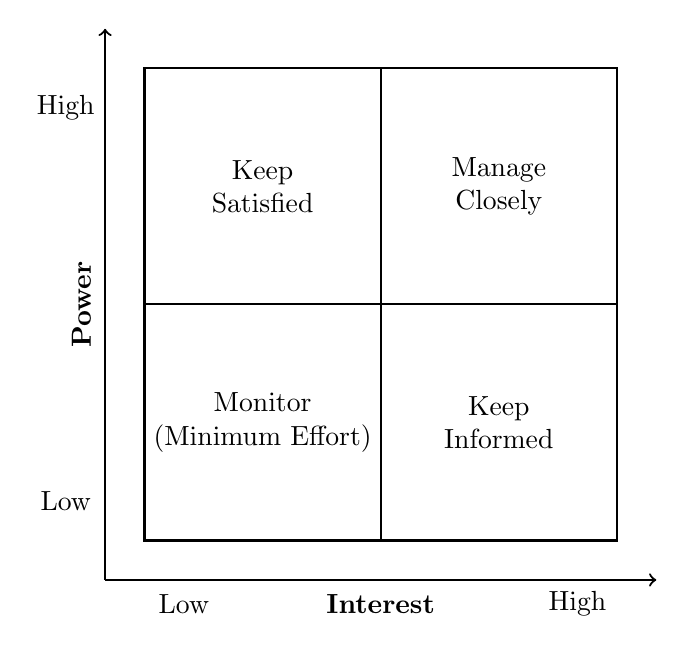
\begin{tikzpicture}
        % Draw grid
        \draw[thick] (0,0) rectangle (6,6);
        \draw[thick] (3,0) -- (3,6);
        \draw[thick] (0,3) -- (6,3);
        
        % Labels
        \node[rotate=90] at (-0.8,3) {\textbf{Power}};
        \node at (3,-0.8) {\textbf{Interest}};

        % Axis labels
        \node at (-1,5.5) {High};
        \node at (-1,0.5) {Low};
        \node at (0.5,-0.8) {Low};
        \node at (5.5,-0.8) {High};

        % Quadrant text using \parbox for multi-line
        \node at (1.5,4.5) {\parbox{3cm}{\centering Keep \\ Satisfied}};
        \node at (4.5,4.5) {\parbox{3cm}{\centering Manage \\ Closely}};
        \node at (1.5,1.5) {\parbox{3cm}{\centering Monitor \\ (Minimum Effort)}};
        \node at (4.5,1.5) {\parbox{3cm}{\centering Keep \\ Informed}};

        % Axes arrows
        \draw[->, thick] (-0.5,-0.5) -- (-0.5,6.5);
        \draw[->, thick] (-0.5,-0.5) -- (6.5,-0.5);

    \end{tikzpicture}
\end{center}

\subsection{Noise impact}
...

\subsubsection{Low frequency noise (LFN)}
...

\subsection{Impact on birds}
...

\subsubsection{Methods to reduce impacts on birds}
...

\subsection{Electromagnetic interference (EMI)}
...

\newpage
\section*{EIA exercise -- 140 MW offshore wind park}

\subsection*{Task 1}
\subsubsection*{What is being proposed?}
\begin{itemize}
    \item 140 MW Offshore Park $\Rightarrow$ 70 turbines (2 MW each), grid pattern
    \item 110 m high turbines (70 m hub height), monopole foundation rammed into seabed
    \item 50 km of interconnecting cables: 36 kV grid, 20 km sea cable to shore, 5 km passing through protected landscape
    \item 4x4 m helicopter landing pad $\times$ 70 turbines
\end{itemize}

\subsubsection*{Why?}
\begin{itemize}
    \item To increase Denmark’s renewable energy capacity and reduce reliance on fossil fuels
    \item To harness strong wind resources in offshore shallow waters for stable electricity generation
    \item To contribute to national and international climate goals by reducing carbon emissions
\end{itemize}

\subsubsection*{Type of Environmental Impact Assessment (EIA)}
\begin{itemize}
    \item Full EIA required due to scale and proximity to protected area
    \item Impact on seabed: marine ecosystems (disruption of benthic habitats)
    \item Noise $\Rightarrow$ interference with marine lifeforms (whales, harbor porpoises, migratory birds)
    \item Visual impact $\Rightarrow$ minor concern (offshore location)
    \item Sediment movement $\Rightarrow$ water quality $\Rightarrow$ potential degradation
    \item Potential methane sink disruption
\end{itemize}

\subsection*{Task 2}
\subsubsection*{Relevant Impact Categories}
\begin{itemize}
    \item Marine ecosystem: impact on fish, marine mammals, and benthic organisms
    \item Bird migration: risk of collision, displacement due to rotor movement
    \item Seabed disturbance: monopile foundation and cable laying altering sediment dynamics
    \item Water quality: increased turbidity due to construction
    \item Underwater noise pollution: pile driving and operational noise
    \item Shipping and navigation safety: potential risks to vessels
    \item Climate benefits: renewable energy reducing CO$_2$ emissions
\end{itemize}

\subsubsection*{Less Important Categories}
\begin{itemize}
    \item Soil erosion (not relevant offshore)
    \item Deforestation (not applicable)
    \item Land-use change (only minor coastal modifications)
\end{itemize}

\subsection*{Task 3}
\subsubsection*{Installation Phase}
\begin{itemize}
    \item Harbor porpoise $\Rightarrow$ hearing impacted by pile-driving noise ($\approx$150 kHz sensitivity)
    \item Sediment resuspension $\Rightarrow$ increased turbidity affecting marine life
    \item Increased vessel traffic $\Rightarrow$ potential collisions with marine animals
    \item Temporary displacement of fish and marine mammals
\end{itemize}

\subsubsection*{Operation Phase}
\begin{itemize}
    \item Bird collisions: seabirds (e.g., gannets, gulls, kittiwakes) impacted
    \item Continuous noise from turbines $\Rightarrow$ communication interference for marine mammals
    \item Creation of artificial reef structures around monopile bases (potential biodiversity benefit)
    \item Reduction of CO$_2$ emissions contributing to climate mitigation
\end{itemize}

\newpage
\part{Environmental impacts - offshore}
\section{Environmental impacts}
\subsection{Visual impact}
...

\begin{center}
    \begin{tabular}{|c|c|}
        \hline
        \multicolumn{2}{|c|}{\textbf{Threshold}}\\
        \hline
        \textbf{Distance} & \textbf{Impact}\\
        \hline
        $<$13 km & possible major visual effects\\
        \hline
        13 -- 24 km & possible moderate visual effects\\
        \hline
        $>$24 km & possible minor visual effects\\
        \hline
    \end{tabular}
\end{center}

\subsection{Noise impact}
...

\subsubsection{Construction phase}
...

\subsubsection{Operation phase}
...

\subsection{Electromagnetic fields}
...

\subsection{Turbine foundation}
...

\subsection{Impact on sea birds}
...

\begin{center}
    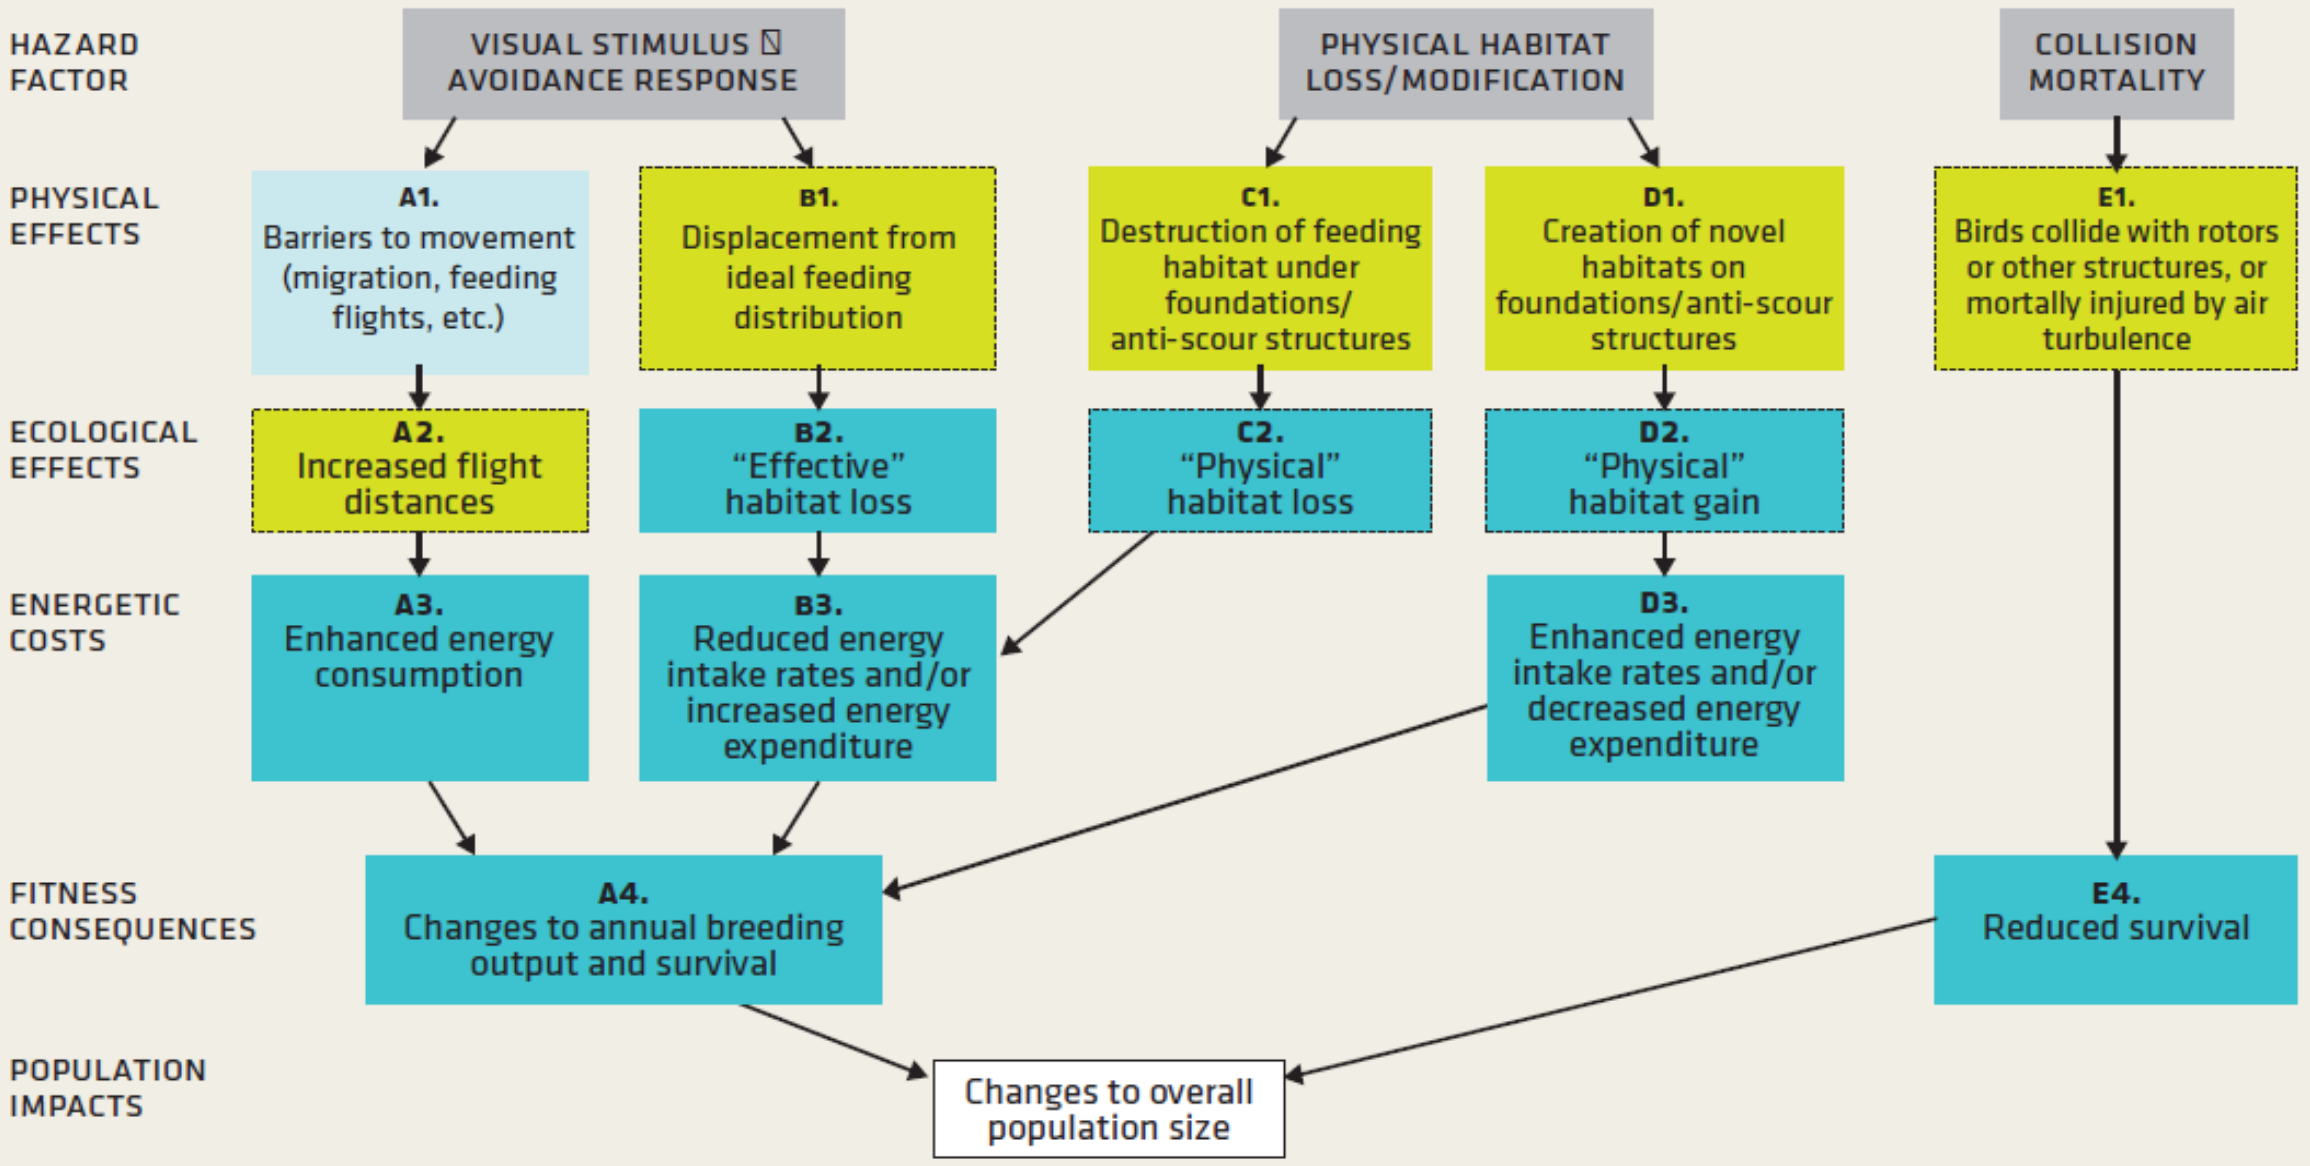
\includegraphics[width=\textwidth]{media/offshore_impact.png}
\end{center}

\subsection{Ship collisions}
...

\subsection{Other impacts}
...

\subsubsection{Radar signals}
...

\subsubsection{Shadowing (masking)}
...

\subsubsection{Returns}
...

\subsubsection{Scattering}
...

\newpage
\part{Cost of windpower}
\section{Wind economics}
\subsection{Cost types}
Cost can be measured in a number of different ways:
\begin{itemize}
    \item Capital (initial investment/equipment) costs;
    \item Operation and maintenance costs;
    \item Levelised cost of enegy (LCOE);
    \item Fixed/variable costs
\end{itemize}

Cost can be measured from different perspectives:
\begin{itemize}
    \item Private investors / Indipendent power producers \tra Cost/financial analysis;
    \item State-owned electricity generation utility \tra Economic analysis:\\
        (e.g.: incl. subsidies, taxation, incentives, CO$_2$ pricing, externalities, ...)
\end{itemize}

\subsection{Private companies}
Benefits:
\begin{itemize}
    \item Energy price (comes from the grid operator);
    \item Sell of energy;
    \item Zero-emission energy \tra best air quality and life quality;
    \item People and families move near the area in order to get job.
\end{itemize}

\subsection{Private companies}
-

\newpage
\section{Levelised cost of electricity generation (LCOE)}
\begin{itemize}
    \item LCOE is a measure of cost effectiveness of a energ source;
    \item It is used to compare different methods of electricity generation on a comparable basis;
    \item LCOE is calculated by accounting for all of a system's expected lifetime costs
        devided by the system's lifetime expected power output (kWh);
    \item LCOE reflects minimum price at which electricity has to be sold (excl. taxes):
        \begin{itemize}[label=$\circ$]
            \item A relatively low LCOE means that electricity is being produced at a low cost;
            \item Higher likely returns for investor;
        \end{itemize}
    \item LCOE of renewable energy rechnologies varies by technology, country and project:
        \begin{itemize}[label=$\circ$]
            \item Depending on energy resource, capital/operating costs and efficiency/performance;
        \end{itemize}
    \item Cost of energy technologies is based on discounting financial flows:
        \begin{itemize}[label=$\circ$]
            \item Discounting: multiplying an amount (cost) by a discount rate to determine its present value;
            \item Discounting is the opposite of compounding;
            \item (e.g.: 1'000.- compounded at annual interest rate of 10\% per year for 5 years = 1'610.51.-)
            \item (inverse: Present value of 1,610.51.- realized ayer 5 years discounted at 10\% per year = 1,000.-)
        \end{itemize}
    \item (e.g.: Cost structure for wind turbines \tra Capital costs, maintenances, deconstruction.)
\end{itemize}

\subsubsection{LCOE formula}
\figbox{LCOE $= \dfrac{\dm \sum_{n}^{t=1} \frac{I_t + M_t + F_t}{(1+r)^t}}{\dm \sum_{n}^{t=1} E_t}$}
where:
\begin{itemize}
    \item \textbf{LCOE} = the average lifetime levelised cost of electricity generation;
    \item $\mathbf{I_t}$ = investment expenditures in the yeat $\mathbf{t}$;
    \item $\mathbf{M_t}$ = operations and maintenance expenditures in the year $\mathbf{t}$;
    \item $\mathbf{F_t}$ = fuel expenditures in the year $\mathbf{t}$;
    \item $\mathbf{E_t}$ = electricity generation in the year $\mathbf{t}$;
    \item $\mathbf{r}$ = discount rate;
    \item $\mathbf{n}$ = economic life of the system.
\end{itemize}

\pph{Example}
A company has a 1mil francs as capital costs and, after 10 years, they have still 1mil francs at the end. The initial costs are higher or lower, considering a big discount rate?

Net costs: Initial Outlay $-$ Present Value of any Return

$\Rightarrow$ $1'000'000 - \dfrac{1'000'000}{(1+r)^{10}}$

When the discount rate is large, the 1 million francs you have at the end of 10 years is heavily discounted and not worth very much in today’s terms. Effectively, that makes your net cost higher.

So, to answer the question directly:\\
They are effectively higher, because you are not getting much present-value ``credit'' for the 1 million francs you receive 10 years in the future.

\subsubsection{Energy LCOE}
\begin{itemize}
    \item Quality of LCOE estimations strongly depends on quality and detail level of input data;
    \item LCOE estimations are tipically characterized by large uncertainity range (e.g.: maintenance costs, produced kWh);
    \item LCOE estimates are highly sensitive to assumed discount rate.
\end{itemize}

\begin{center}
    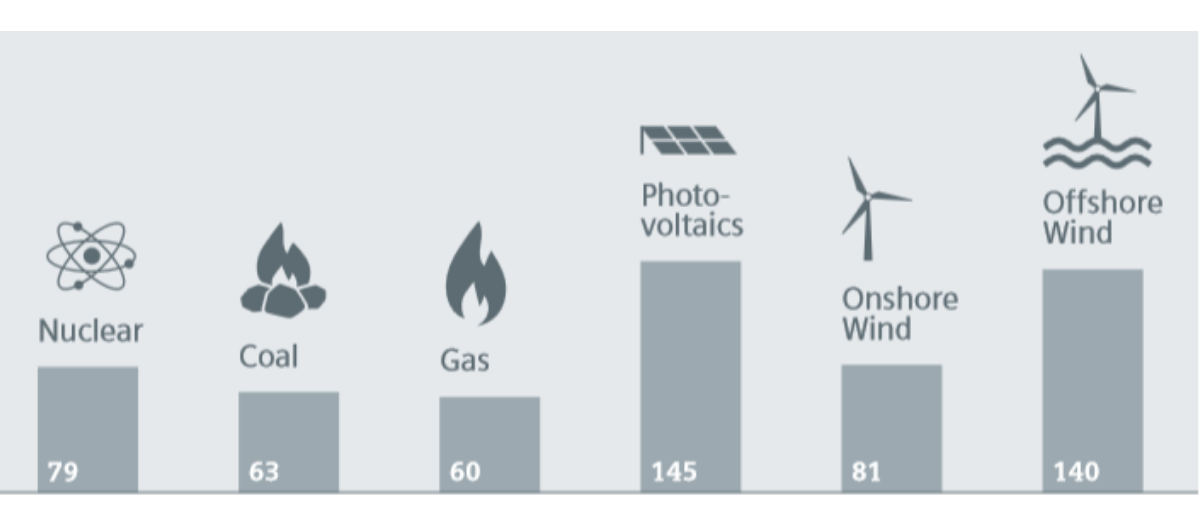
\includegraphics[width=.8\textwidth]{media/energy_lcoe.png}
\figbox{LCOE $= \dfrac{\text{Total costs over lifetime [\textcurrency]}}{\text{Electricity produced over lifetime [kWh]}}$}
\end{center}

\subsubsection{Guidance scheme}
EU guidance scheme for LCOE best practice:
Guidelines defines minimum cost parameters that should be included in LCOE calculation:
\begin{itemize}
    \item ...
\end{itemize}

\subsection{Capital (investment) cost}
\subsubsection{Investments}
\begin{itemize}
    \item Cost structure of a wind power project is dominated by upfront capital cost:
    \begin{itemize}[label=$\circ$]
        \item Up to 70--80\% of total cost;
        \item No fuel price risk during operation;
    \end{itemize}
    \item Capital costs of a wind power project can be broken down into:
    \begin{itemize}[label=$\circ$]
        \item Turbine cost (incl. blades, tower and transformer);
        \item Civil works (incl. construction costs for site preparation, foundation construction);
        \item Grid connection costs (incl. transformers, substations, connection to transmissio network);
        \item Other capital costs (e.g.: construction of buildings, project consultancy costs, ...).
    \end{itemize}
\end{itemize}

\begin{center}
    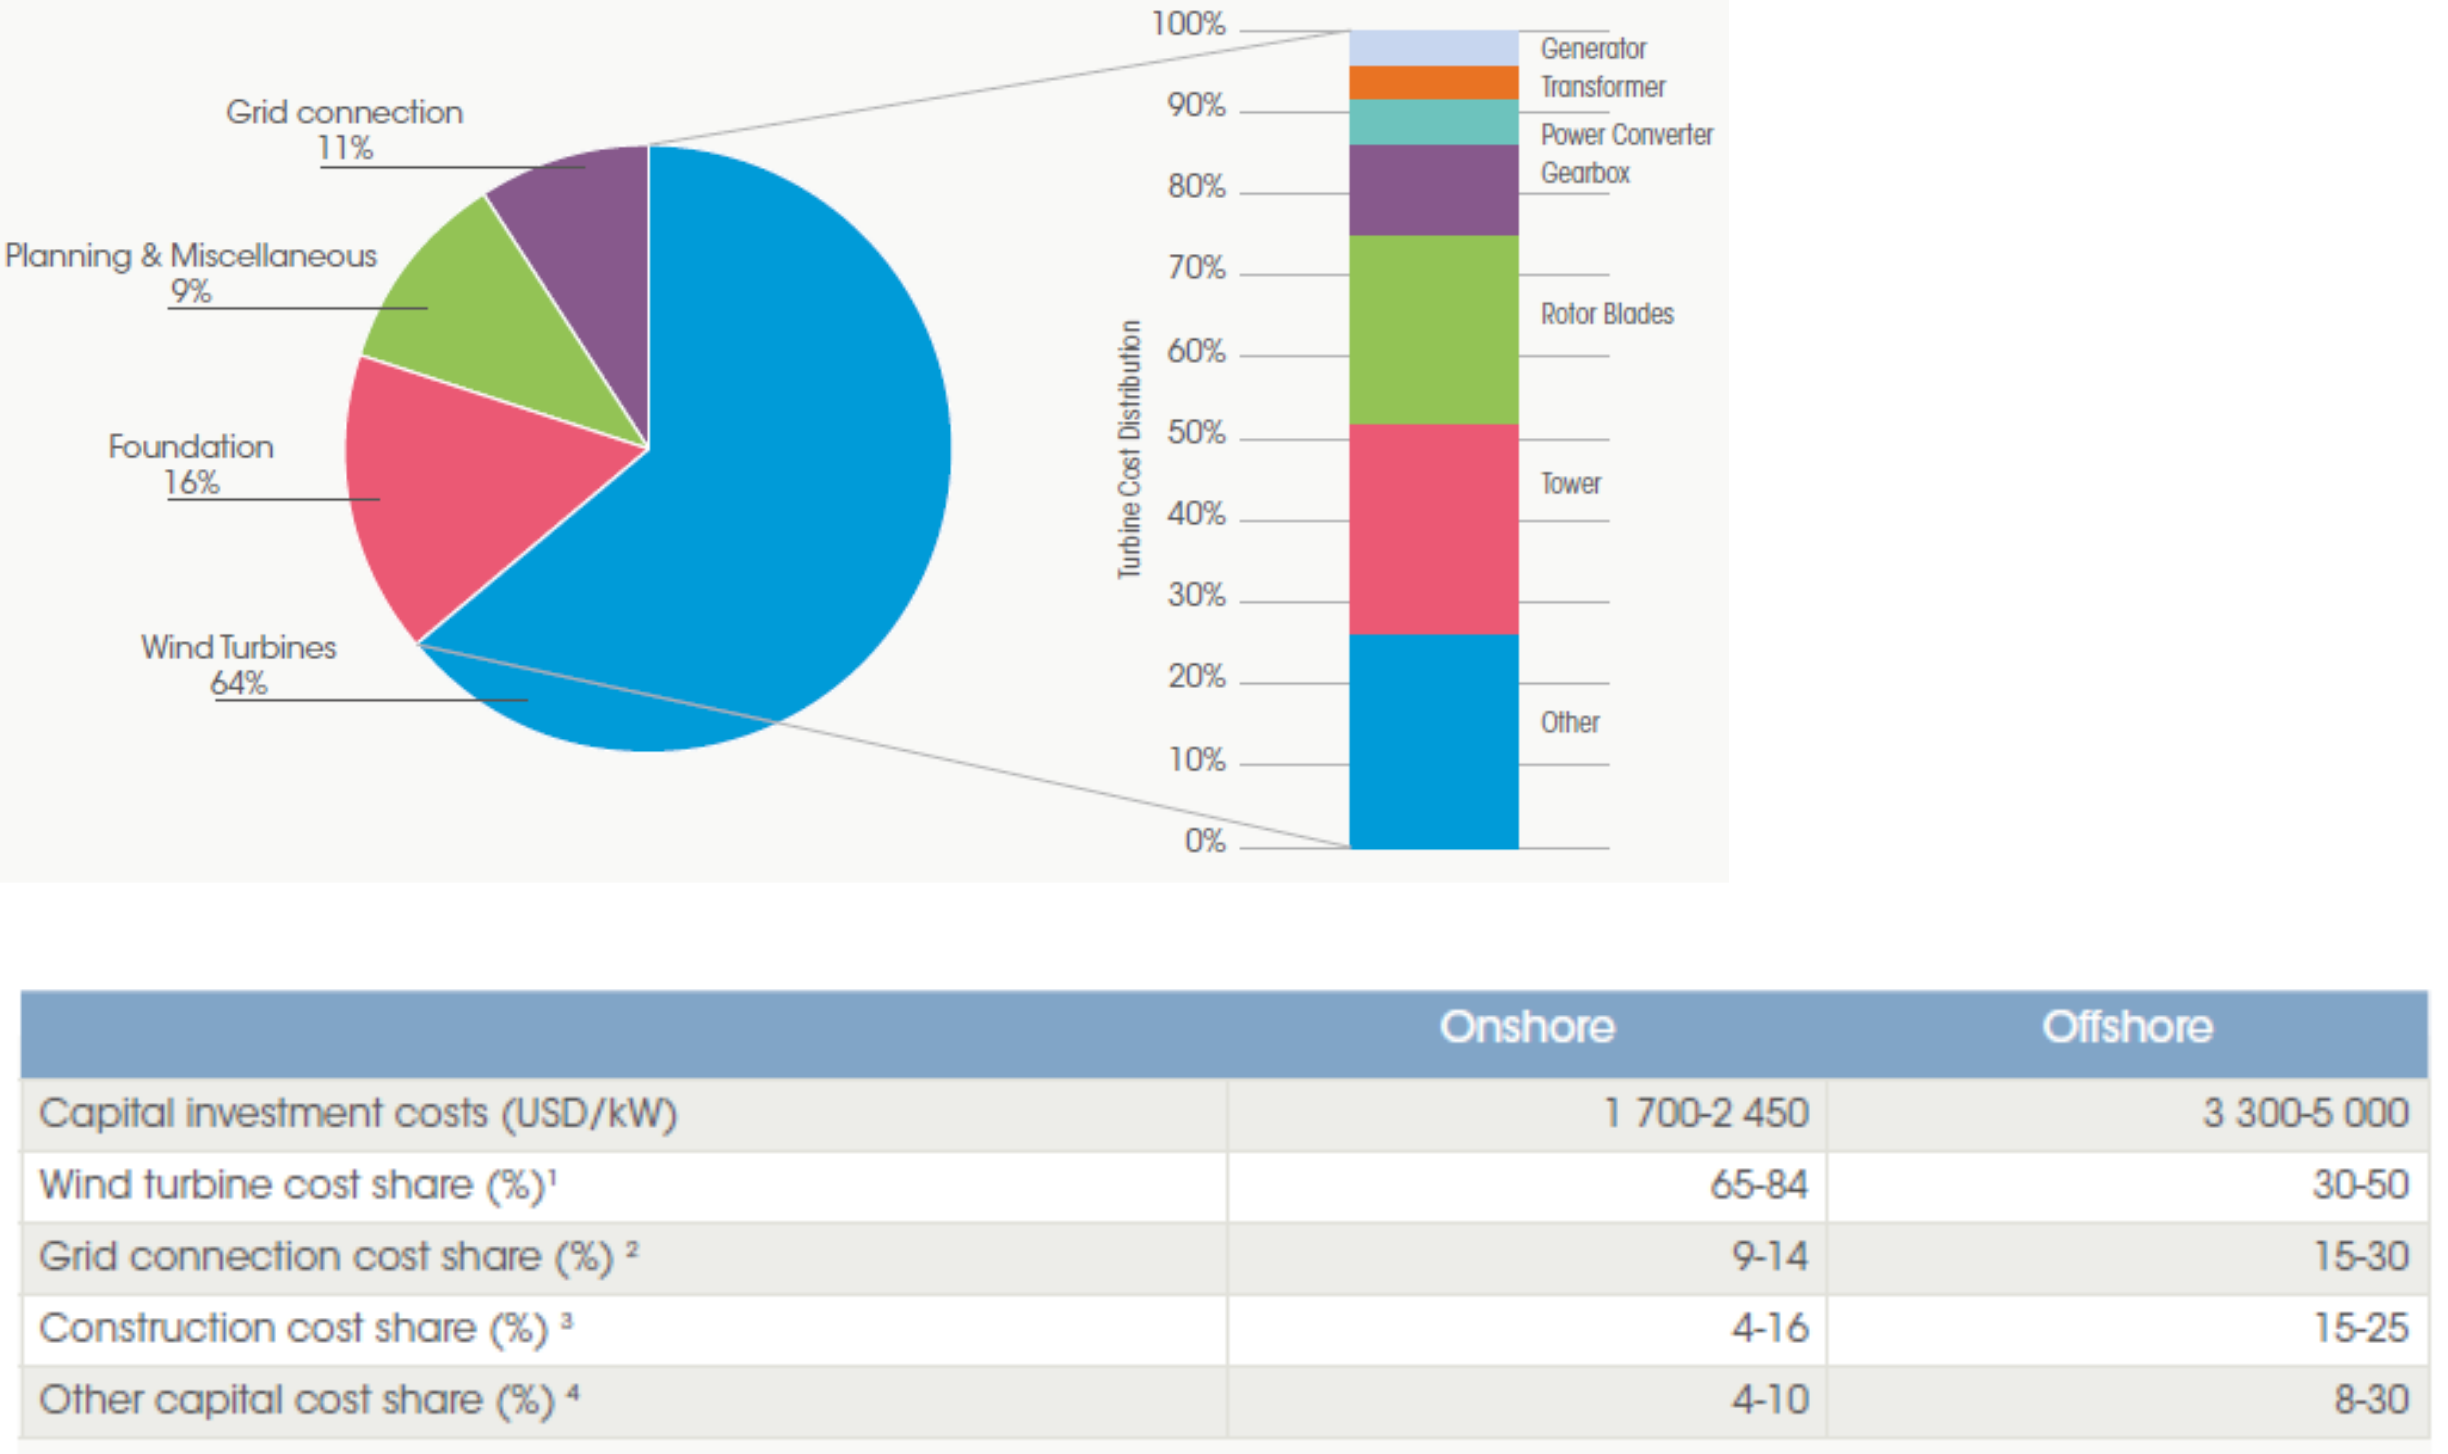
\includegraphics[width=\textwidth]{media/investment.png}
\end{center}

Share of different cost components varies by country and project:
\begin{itemize}
    \item Country specific cost structure (e.g. labour cost, land cost etc.);
    \item Project specific cost structure (type and size of turbine, off- or onshore etc.).
\end{itemize}

\begin{center}
    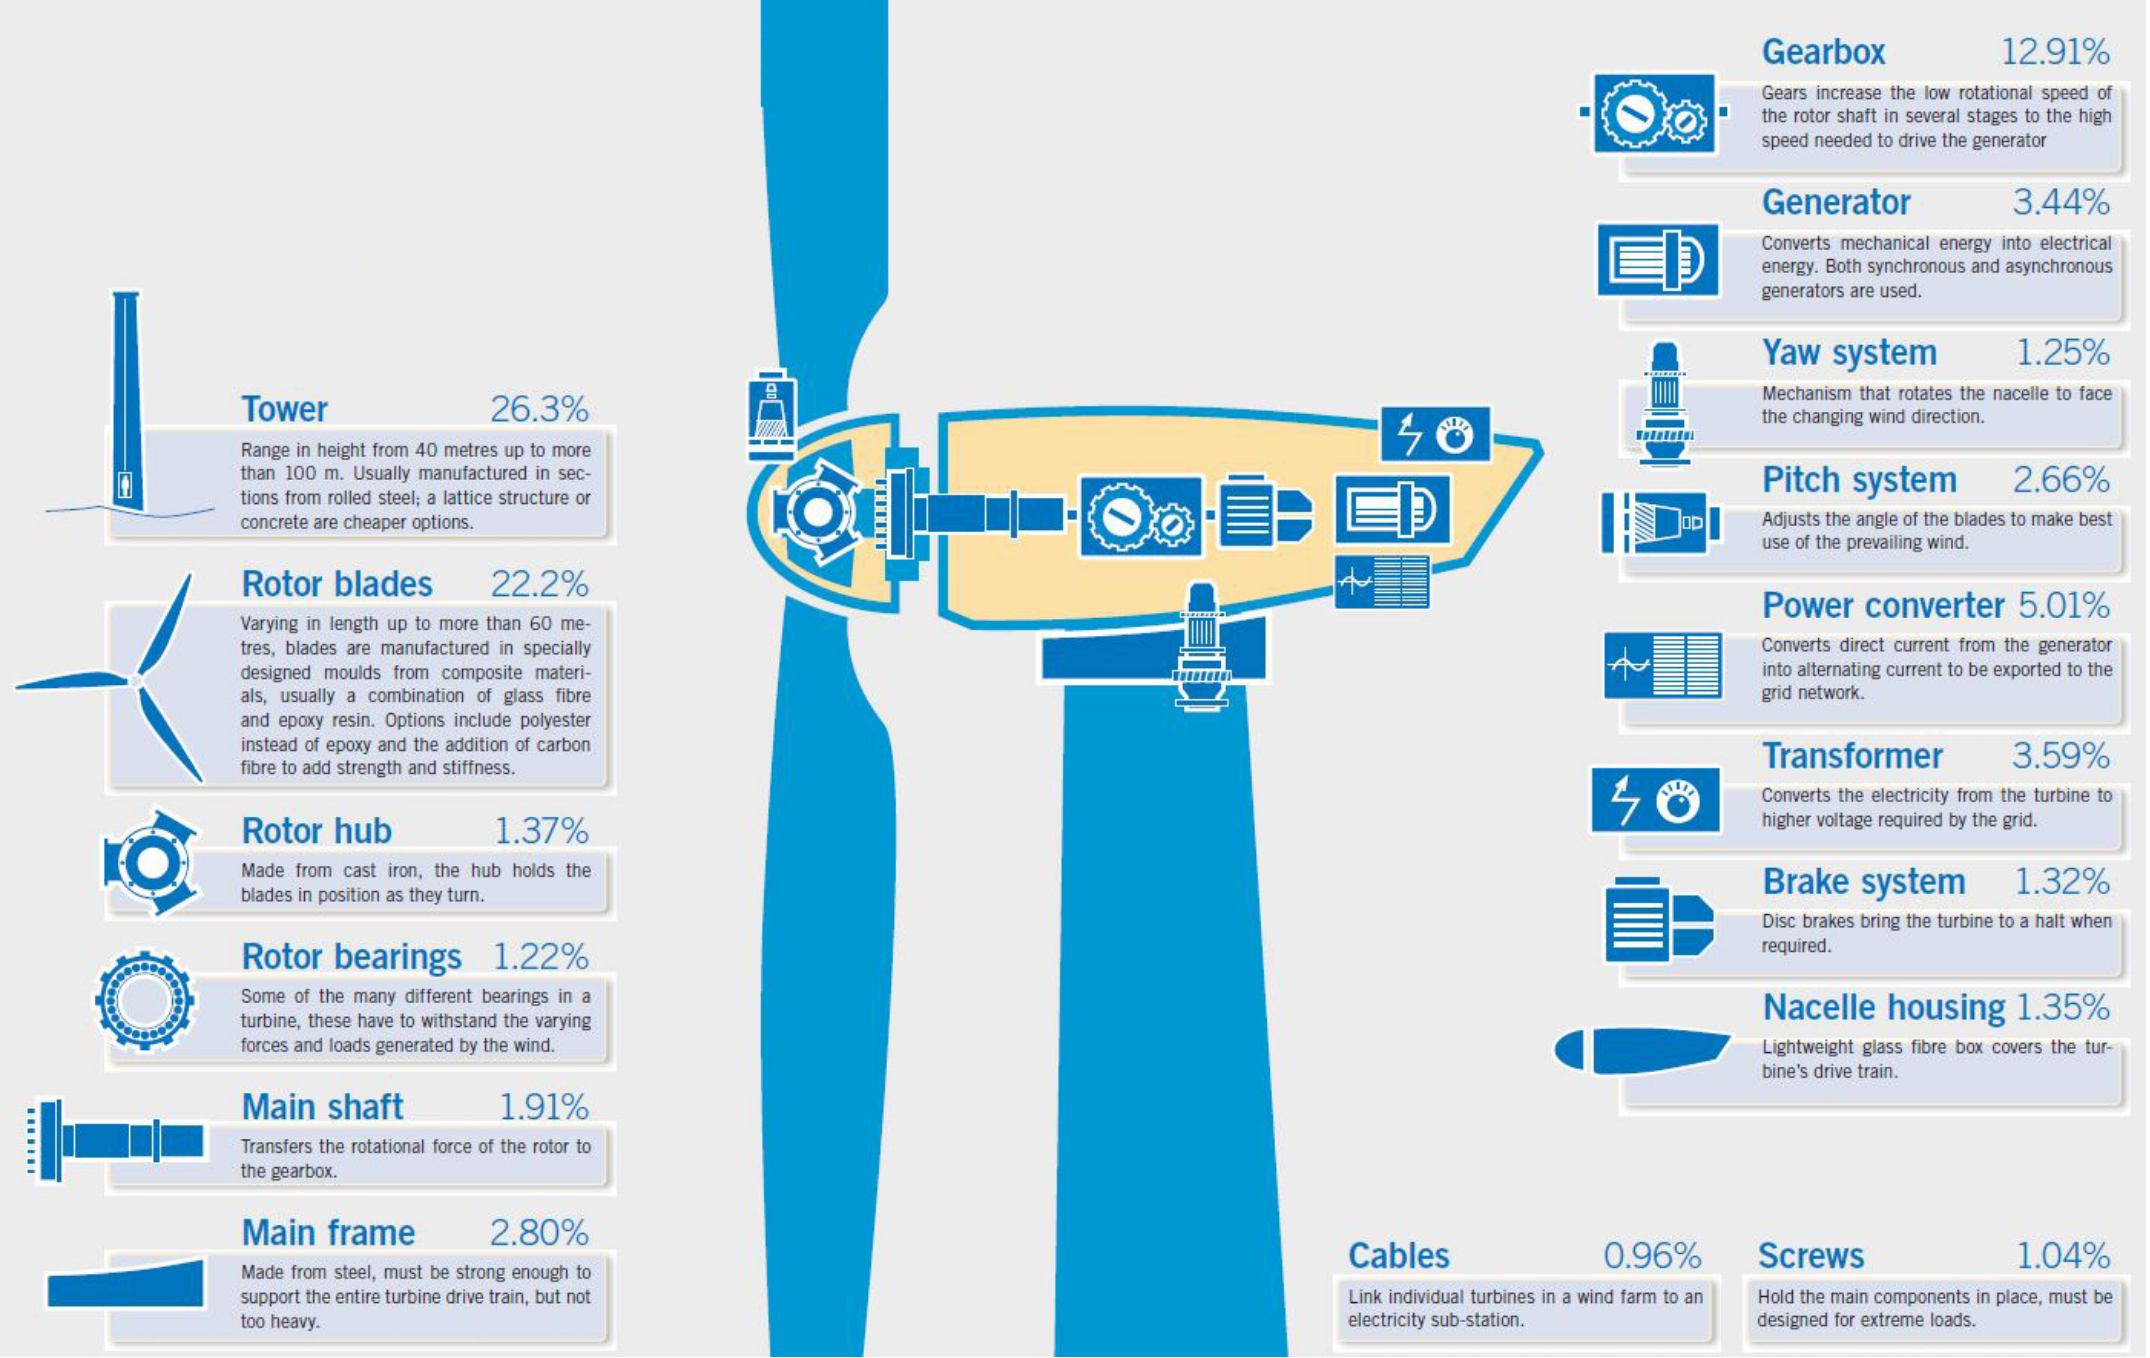
\includegraphics[width=\textwidth]{media/eolic_turbine.png}
\end{center}

\begin{itemize}
    \item Investment cost of onshore wind power projects in developed countries:
    \begin{itemize}[label=$\circ$]
        \item Range between USD 1,700/kW - USD 2,400/kW;
        \item In comparison in China capital costs are around USD 1,300/kW;
    \end{itemize}
    \item During 1980 and 2004 capital costs steadily declined;
    \item Ayer 2004 installed cost increased to around USD 2,000/kW;
    \item Reasons for price increases are include:
    \begin{itemize}[label=$\circ$]
        \item Rising cost of commodities (e.g. steel, copper);
        \item Copper and steel account for around 20-40\% of total capital cost;
        \item High market demand lead to shortages in certain components \tra higher prices;
    \end{itemize}
    \item Capital costs for offshore wind projects in developed countries:
    \begin{itemize}[label=$\circ$]
        \item Vary between USD 3,300 - USD 5,000/kW;
        \item Price variation depending on water depth - shiy from a shallow to deeper water projects.
    \end{itemize}
\end{itemize}

\subsection{O\&M cost}
...

\subsection{Cost reduction potential}
\subsubsection{Turbine components}
...

\subsubsection{Grid connection}
\begin{itemize}
    \item Cost of grid connection is not likely to decline significantly for onshore wind farms;
    \item Offshore grid connection costs can be reduced by increased scale of wind parks.
\end{itemize}

\subsubsection{Foundation}
\begin{itemize}
    \item Foundations accounts for 7-10\% of onshore costs;
    \item 15\% to 20\% for offshore costs;
    \item Largest cost components are cement and steel;
    \item Cost reductions by reduced material consumption (more efficient design);
    \item Cost reductions by reduced materials cost or materials substitution;
    \item Cost reduction by new offshore foundation designs \tra Fixed seabed vs. floating foundation (in testing stage).
\end{itemize}
 
\subsubsection{Other}
...

\subsection{Levelised cost of electricity from wind energy}
...

\newpage

















\end{document}